\chapter{SmartCGMS}

SmartCGMS je systém kontinuální monitorace glukózy nové generace vyvíjený na Katedře informatiky a výpočetní techniky na Fakultě aplikovaných věd Západočeské univerzity v Plzni. Umožňuje kontinuální monitoraci glukózy, modelování dynamiky glukózy a řízení inzulinové pumpy.

Aplikace je napsaná v jazyce C++ a je zkompilována pro x86-64 systémy MS Windows, macOS, Debian GNU/Linux a pro armeabi-v7a a arm64-v8a \citep{cgms.koutny}. Skládá se z filtrů, modelů, metrik a solverů.

\textbf{Filtr} je základní stavební prvek aplikace, který poskytuje určitou funkcionalitu. Ty mají jednotné rozhraní a jsou poskládány lineárně za sebou (viz příklad konfigurace na obrázku \ref{fig:scgms_filters}). To umožňuje vysokou modularitu a zaměnitelnost filtrů (například filtr, který čte data ze senzoru CGMS, se může nahradit filtrem, který přečte data uložená v logu, bez nutnosti změn ve zbytku konfigurace). Filtry spolu komunikují předáváním událostí. Událost obsahuje typ události (level, info, parameters), id filtru, který událost vytvořil, typ signálu, hodnotu, časový segment a čas vytvoření události. Nejčastější je událost typu level, která v sobě má hodnotu naměřeného nebo vypočteného signálu. Události se zpracovávají postupně tak, jak přichází. Filtr může událost poslat dál beze změny, událost upravit, nebo událost zahodit a případně vygenerovat nový signál.

\begin{figure}[H]
\caption{Příklad konfigurace filtrů SmartCGMS}
\label{fig:scgms_filters}
\centering
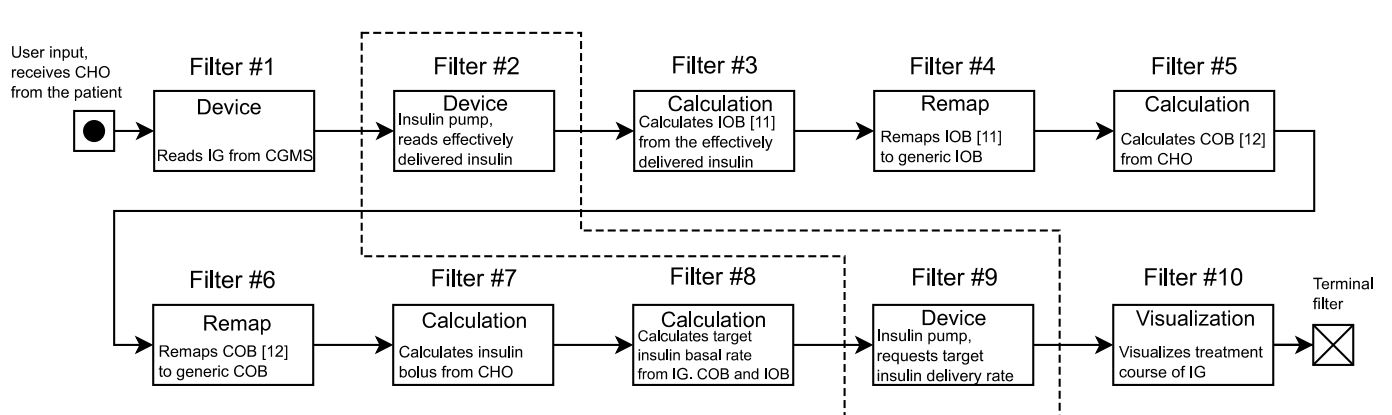
\includegraphics[width=1\textwidth]{img/scgms/filters.jpg}
\textit{Zdroj: SmartCGMS as an Environment for an Insulin-Pump  Development with FDA-Accepted In-Silico Pre-Clinical Trials \citep{cgms.ubl}}
\end{figure}

\textbf{Model} umožňuje načtení více hodnot a jejich následné zpracování dle nastavených parametrů. Narozdíl od filtru model zpracovává události dávkově. Je tak vhodný pokud potřebujeme pracovat s více signály najednou nebo predikovat hodnotu do budoucna. SmartCGMS obsahuje modely dynamiky glukózy Bergmanův model vylepšený Hovorkovo modelem a Koutného difúzním modelem, SimGlucose s vynulovaným parametrem xi u UVA/Padova S2013, T1DMS a DMMS.R \citep{cgms.web}. Výpočet modelu je spušten filtrem \textit{Signal Generator} nebo filtrem \textit{Calculated Signal}, pokud chceme  parametry modelu dynamicky spočítat pomocí solveru.

\textbf{Metrika} je druh filtru, který umožňuje spočítat metriky jako je například střední chyba, směrodatná odchylka nebo plocha pod křivkou \citep{cgms.koutny}.

Pro určení parametrů modelu lze využít \textbf{solver}. Ten na základě metrik signálů modelu spočítá jeho optimální parametry. Příkladem solveru je Meta-differential evolution, Pathfinder, Sequential brute force scan, Particle swarm optimization, Spiral optimization a další.

Vytvořené filtry, modely a solvery se zkompilují jako dynamická knihovna, která se načte při spuštění SmartCGMS. Aplikace také umožňuje integraci skriptů v jazyce Matlab. Skripty je nutné definovat v souboru \textit{matlab\_manifest.xml}.

SmartCGMS lze spustit v příkazové řádce (\textit{console3.exe}) nebo v grafickém uživatelském rozhraní (\textit{gpredict3.exe}). V záložce \textit{Filters} si uživatel nastaví jednotlivé filtry a jejich parametry. V záložce \textit{Simulation} pak spustí běh programu a může prohlížet grafy a logy s výstupy (příklad grafického výstupu je na obrázku \ref{fig:scgms_graf}). Konfiguraci lze uložit a poté opětovně načíst.

SmartCGMS je dostupný na \url{https://diabetes.zcu.cz/smartcgms}.

\begin{figure}[H]
\caption{Příklad výstupu SmartCGMS}
\label{fig:scgms_graf}
\centering
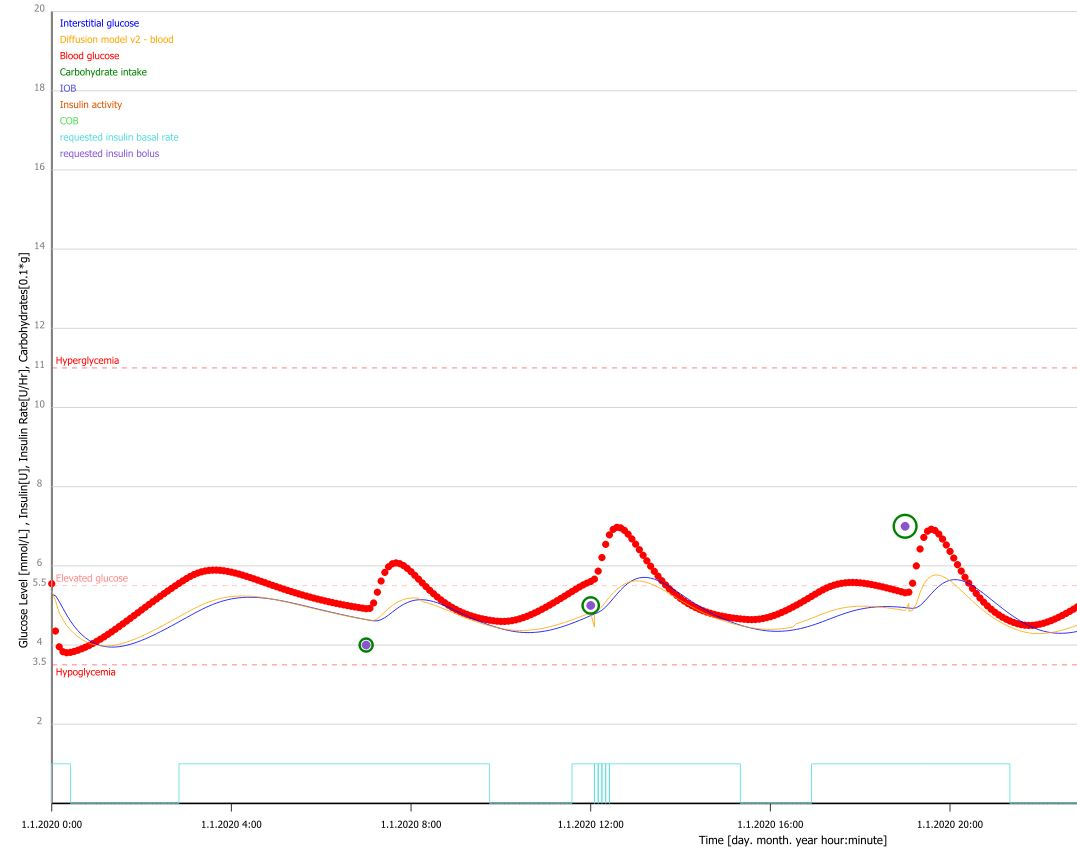
\includegraphics[width=1\textwidth]{img/scgms/graf1.jpg}
\textit{Zdroj: SmartCGMS}
\end{figure}